\chapter{Толық ізденіс}

\key{Толық ізденіс} -- кез келген алгоритмдік есепті шығарудың 
жалпылама түрі. Негізгі идеясы толықтай іріктеуді қолдана отырып, барлық
мүмкін жауаптарды қарастыруға, кейін есеп шартына байланысты ең үздік
нәтижелерді іріктеу немесе шешімдер санын есептеуге бағытталады.

Толық ізденісті барлық мүмкін шешімдерді қарастыруға уақыт жеткілікті болғанда ғана
тиімді әдіс деп есептеуге болады, себебі мұндай ізденіс әдетте оңай орындалады және әрдайым
дұрыс жауапты көрсетеді. Егер толық ізденіс тым баяу болса, ашкөз алгоритмдер немесе 
динамикалық бағдарламалау сияқты өзге әдіс-тәсілдер қажет болуы мүмкін.

\section{Ішжиындар құру}

\index{ішжиын}

Бірінші қарастыратын есебіміз  $n$ элементтен тұратын
жиынның барлық ішжиындарын құруға арналады.
Мысалы, $\{0,1,2\}$ ішжиындары:
$\emptyset$, $\{0\}$, $\{1\}$, $\{2\}$, $\{0,1\}$,
$\{0,2\}$, $\{1,2\}$ және $\{0,1,2\}$.
Ішжиындарды құрудың негізгі екі әдісі бар. Олар:
не рекурсивті ізденіс жүргізу, не бүтін сандардың 
биттік көрсетілімін қолдану.
% we can either perform a recursive search
% or exploit the bit representation of integers.

\subsubsection{1-әдіс}

Жиындағы барлық ішжиындарды өтіп шығудың ыңғайлы жолы -- рекурсия.
Келесі \texttt{search} функциясы $\{0,1,\ldots,n-1\}$ жиынының
ішжиындарын құрастырады. Функция әр ішжиынның элементтерін сақтайтын
\texttt{subset} векторын қолдайды. Ізденіс функциясы 0 параметрімен шақырылғаннан кейін
басталады.

\begin{lstlisting}
void search(int k) {
    if (k == n) {
        // process subset
    } else {
        search(k+1);
        subset.push_back(k);
        search(k+1);
        subset.pop_back();
    }
}
\end{lstlisting}

\texttt{search} функциясы $k$ параметрімен шақырылғанда
ішжиынға $k$ элементін қосу, не қоспау туралы шешім қабылдайды,
екі жағдайда да өзін $k+1$ параметрімен қайта шақырады.
Дегенмен, егер $k=n$ орындалса, функция барлық элементтер 
қаралғанын және ішжиын құрылғанын байқайды.

Төмендегі дарақ $n=3$ болған жағдайдағы шақыруларды көрсетеді.
Біз әрдайым не сол тармақты
($k$ ішжиымға кірмейді), не оң тармақты 
($k$ ішжиымға кіреді) таңдай аламыз.

\begin{center}
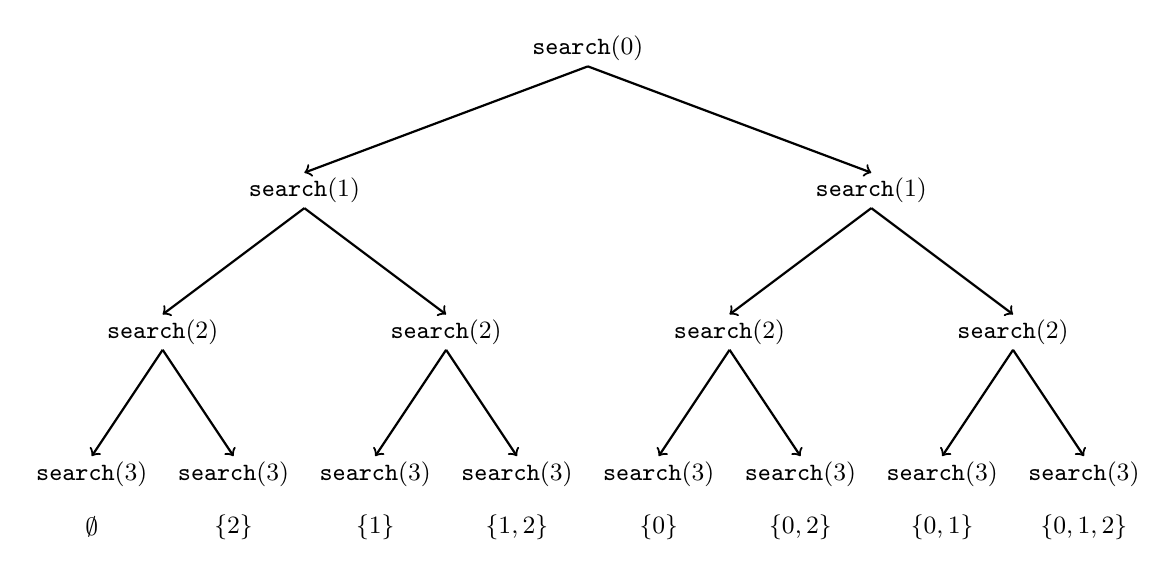
\begin{tikzpicture}[scale=.45]
  \begin{scope}
    \small
    \node at (0,0) {$\texttt{search}(0)$};

    \node at (-8,-4) {$\texttt{search}(1)$};
    \node at (8,-4) {$\texttt{search}(1)$};

    \path[draw,thick,->] (0,0-0.5) -- (-8,-4+0.5);
    \path[draw,thick,->] (0,0-0.5) -- (8,-4+0.5);

    \node at (-12,-8) {$\texttt{search}(2)$};
    \node at (-4,-8) {$\texttt{search}(2)$};
    \node at (4,-8) {$\texttt{search}(2)$};
    \node at (12,-8) {$\texttt{search}(2)$};

    \path[draw,thick,->] (-8,-4-0.5) -- (-12,-8+0.5);
    \path[draw,thick,->] (-8,-4-0.5) -- (-4,-8+0.5);
    \path[draw,thick,->] (8,-4-0.5) -- (4,-8+0.5);
    \path[draw,thick,->] (8,-4-0.5) -- (12,-8+0.5);

    \node at (-14,-12) {$\texttt{search}(3)$};
    \node at (-10,-12) {$\texttt{search}(3)$};
    \node at (-6,-12) {$\texttt{search}(3)$};
    \node at (-2,-12) {$\texttt{search}(3)$};
    \node at (2,-12) {$\texttt{search}(3)$};
    \node at (6,-12) {$\texttt{search}(3)$};
    \node at (10,-12) {$\texttt{search}(3)$};
    \node at (14,-12) {$\texttt{search}(3)$};

    \node at (-14,-13.5) {$\emptyset$};
    \node at (-10,-13.5) {$\{2\}$};
    \node at (-6,-13.5) {$\{1\}$};
    \node at (-2,-13.5) {$\{1,2\}$};
    \node at (2,-13.5) {$\{0\}$};
    \node at (6,-13.5) {$\{0,2\}$};
    \node at (10,-13.5) {$\{0,1\}$};
    \node at (14,-13.5) {$\{0,1,2\}$};


    \path[draw,thick,->] (-12,-8-0.5) -- (-14,-12+0.5);
    \path[draw,thick,->] (-12,-8-0.5) -- (-10,-12+0.5);
    \path[draw,thick,->] (-4,-8-0.5) -- (-6,-12+0.5);
    \path[draw,thick,->] (-4,-8-0.5) -- (-2,-12+0.5);
    \path[draw,thick,->] (4,-8-0.5) -- (2,-12+0.5);
    \path[draw,thick,->] (4,-8-0.5) -- (6,-12+0.5);
    \path[draw,thick,->] (12,-8-0.5) -- (10,-12+0.5);
    \path[draw,thick,->] (12,-8-0.5) -- (14,-12+0.5);
\end{scope}
\end{tikzpicture}
\end{center}

\subsubsection{2-әдіс}

Ішжиындарды құраудың бүтін сандардың биттік көрсетіліміне негізделген жолы да бар. 
$n$ элементтен тұратын жиынның әр ішжиыны $n$ биттен тұратын тізбек ретінде көрсетіле алады,
ол өз кезегінде $0 \ldots 2^n-1$ аралығындағы бүтін сан болады.
% Each subset of a set of $n$ elements
% can be represented as a sequence of $n$ bits,
% which corresponds to an integer between $0 \ldots 2^n-1$.
Бит тізбегіндегі бірліктер қай элементтің ішжиынға кіретіндігін білдіреді.

Әдетте ең соңғы бит 0-элементке, 
ал соңғының алдындағы бит 1-элементке сәйкстендіріледі 
және солай жалғаса береді.
Мысалы, 25 санының биттік көрсетілімі -- 11001,
осылайша біздің ішжиымымыз $\{0,3,4\}$ болмақшы.

Келесі код $n$ элементтен тұратын жиынның ішжиындарымен өтіп шығады:

\begin{lstlisting}
for (int b = 0; b < (1<<n); b++) {
    // process subset 
}
\end{lstlisting}

Келесі код бит тізбегіне сәйкес элементтерден тұратын ішжиынды
қалай табуға болатындағын көрсетеді. Әр ішжиынды өңдеу барысында 
код ішжиын элементтерін сақтайтын вектор құрайды.

\begin{lstlisting}
for (int b = 0; b < (1<<n); b++) {
    vector<int> subset;
    for (int i = 0; i < n; i++) {
        if (b&(1<<i)) subset.push_back(i);
    }
}
\end{lstlisting}

\section{Алмастырулар құрау}

\index{алмастыру}

Біз қарастыратын келесі мәселе -- $n$ элементтен тұратын
жиынның барлық алмастыруларын құрау. Мысалы, $\{0,1,2\}$ алмастырулары --
$(0,1,2)$, $(0,2,1)$, $(1,0,2)$, $(1,2,0)$,
$(2,0,1)$ мен $(2,1,0)$ түрінде жалғасады. Мұндай алмастырулар да екі түрлі амалмен жасалады. Олар:
рекурсияны қолдану немесе алмастыруларды итеративті өтіп шығу.

\subsubsection{1-әдіс}

Ішжиындар сияқты алмастырулар да рекурсивті құрала алады.
Келесі \texttt{search} функциясы $\{0,1,\ldots,n-1\}$ жиынының алмастыруларымен
өтіп шығады. Функция алмастыруды сақтайтын \texttt{permutation} векторын құрады,
ізденіс параметрлерсіз шақырылған функция арқылы басталады.

\begin{lstlisting}
void search() {
    if (permutation.size() == n) {
        // process permutation
    } else {
        for (int i = 0; i < n; i++) {
            if (chosen[i]) continue;
            chosen[i] = true;
            permutation.push_back(i);
            search();
            chosen[i] = false;
            permutation.pop_back();
        }
    }
}
\end{lstlisting}

Әр шақырту \texttt{permutation}-ге жаңа элемент қосады.
\texttt{chosen} жиымы қай элементтердің араластыруға әлдеқашан қосылғандығы туралы хабар береді.
Егер \texttt{permutation} өлшемі жиын өлшемімен теңессе, алмастыру құралғандығын білдіреді.

\subsubsection{2-әдіс}

\index{next\_permutation@\texttt{next\_permutation}}

Алмастыруларды құраудың тағы бір жолына -- 
$\{0,1,\ldots,n-1\}$ алмастыруымен басталып, 
келесі алмастыруды өсу реттілігінде құрастыратын функцияны бірнеше рет шақыру жатады.
Бұл үшін C++ стандартты дерекханасындағы \texttt{next\_permutation} 
функциясын қолдануға болады:

\begin{lstlisting}
vector<int> permutation;
for (int i = 0; i < n; i++) {
    permutation.push_back(i);
}
do {
    // process permutation 
} while (next_permutation(permutation.begin(),permutation.end()));
\end{lstlisting}

\section{Қайта іздеу алгоритмі}

\index{қайта іздеу алгоритмі}

\key{Қайта іздеу (backtracking)} алгоритмі
бос шешіммен басталып, бірте-бірте шешімді кеңейтеді.
Ізденіс рекурсивті түрде шешімнің өзгеруі мүмкін барлық
жолдарын қарастырады.

\index{Уәзір есебі}

Үлгі ретінде $n$ уәзірдің $n \times n$ шахмат тақтасында 
бір-біріне шабуыл жасамайтындай етіп орналастыру жолдарын табу туралы есепті   
қарастырайық. Мысалы, $n=4$ болған жағдайда екі шешім ұсынылады:

\begin{center}
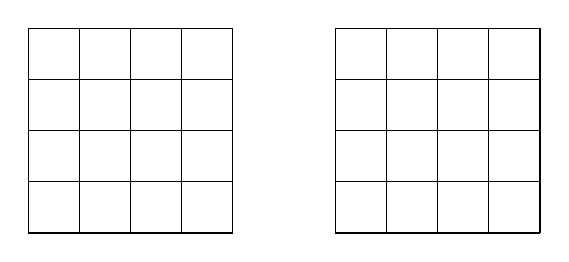
\begin{tikzpicture}[scale=.65]
  \begin{scope}
    \draw (0, 0) grid (4, 4);
    \node at (1.5,3.5) {\symqueen};
    \node at (3.5,2.5) {\symqueen};
    \node at (0.5,1.5) {\symqueen};
    \node at (2.5,0.5) {\symqueen};

    \draw (6, 0) grid (10, 4);
    \node at (6+2.5,3.5) {\symqueen};
    \node at (6+0.5,2.5) {\symqueen};
    \node at (6+3.5,1.5) {\symqueen};
    \node at (6+1.5,0.5) {\symqueen};

  \end{scope}
\end{tikzpicture}
\end{center}

Есепті қайта іздеу алгоритмінің көмегімен 
уәзірді тақтада қатар-қатар орналастыру арқылы
шеше аламыз. Нақтырақ айтсақ, әр қатарға
оған дейін тұрған басқа уәзірлерге шабуыл
жасамайтындай етіп бір ғана уәзір орналастырылады.
Шешім барлық $n$ уәзір орналастырылғаннан кейін
табылады. 

Мысалы, төменде қайта іздеу алгоритмін қолдану арқылы $n=4$ болған жағдайда табылған
кей шешімдер көрсетілген:

\begin{center}
\begin{tikzpicture}[scale=.55]
  \begin{scope}
    \draw (0, 0) grid (4, 4);

    \draw (-9, -6) grid (-5, -2);
    \draw (-3, -6) grid (1, -2);
    \draw (3, -6) grid (7, -2);
    \draw (9, -6) grid (13, -2);

    \node at (-9+0.5,-3+0.5) {\symqueen};
    \node at (-3+1+0.5,-3+0.5) {\symqueen};
    \node at (3+2+0.5,-3+0.5) {\symqueen};
    \node at (9+3+0.5,-3+0.5) {\symqueen};

    \draw (2,0) -- (-7,-2);
    \draw (2,0) -- (-1,-2);
    \draw (2,0) -- (5,-2);
    \draw (2,0) -- (11,-2);

    \draw (-11, -12) grid (-7, -8);
    \draw (-6, -12) grid (-2, -8);
    \draw (-1, -12) grid (3, -8);
    \draw (4, -12) grid (8, -8);
    \draw[white] (11, -12) grid (15, -8);
    \node at (-11+1+0.5,-9+0.5) {\symqueen};
    \node at (-6+1+0.5,-9+0.5) {\symqueen};
    \node at (-1+1+0.5,-9+0.5) {\symqueen};
    \node at (4+1+0.5,-9+0.5) {\symqueen};
    \node at (-11+0+0.5,-10+0.5) {\symqueen};
    \node at (-6+1+0.5,-10+0.5) {\symqueen};
    \node at (-1+2+0.5,-10+0.5) {\symqueen};
    \node at (4+3+0.5,-10+0.5) {\symqueen};

    \draw (-1,-6) -- (-9,-8);
    \draw (-1,-6) -- (-4,-8);
    \draw (-1,-6) -- (1,-8);
    \draw (-1,-6) -- (6,-8);

    \node at (-9,-13) {жарамсыз};
    \node at (-4,-13) {жарамсыз}; 
    \node at (1,-13) {жарамсыз}; 
    \node at (6,-13) {жарамды};

  \end{scope}
\end{tikzpicture}
\end{center}

Ең төменгі деңгейдегі алғашқы үш конфигурация
жарамсыз, өйткені мұндай жағдайда уәзірлер бір-біріне шабуыл жасайды.
Дегенмен төртінші конфигурация жарамды және тақтада
тағы екі уәзірді орналастыру арқылы толық шешімге
кеңейтіле алады. Қалған екі уәзірді орналастырудың
бір ғана жолы бар.

\begin{samepage}
Алгоритмнің жүзеге асырылу жолы:
\begin{lstlisting}
void search(int y) {
    if (y == n) {
        count++;
        return;
    }
    for (int x = 0; x < n; x++) {
        if (column[x] || diag1[x+y] || diag2[x-y+n-1]) continue;
        column[x] = diag1[x+y] = diag2[x-y+n-1] = 1;
        search(y+1);
        column[x] = diag1[x+y] = diag2[x-y+n-1] = 0;
    }
}
\end{lstlisting}
\end{samepage}
Ізденіс \texttt{search(0)} шақыруымен басталады.
Тақтаның өлшемі -- $n \times n$, шешімдер саны
\texttt{count}-та сақталады.

Код тақтадағы бағандар мен қатарлар 0-ден $n-1$-ге дейін
нөмірленген деп есептейді. \texttt{search} функциясы 
$y$ параметрімен шақырылғанда уәзір $y$ қатарына орналастырылады,
кейін өзін $y+1$ параметрімен шақырады. Егер $y=n$ болса, шешім
табылғанын білдіреді және \texttt{count} айнымалысы бірге артады.

\texttt{column} жиымы уәзірі бар бағандарды,
ал \texttt{diag1} және \texttt{diag2} жиымдары 
уәзірі бар диагональдарды сақтайды.  
Уәзірі бұрыннан бар диагональға немесе бағанға тағы бір уәзір
қоса алмаймыз. Мысалы, $4 \times 4$ өлшемді тақтаның диагональдары
мен бағандары осылай нөмірленген:

\begin{center}
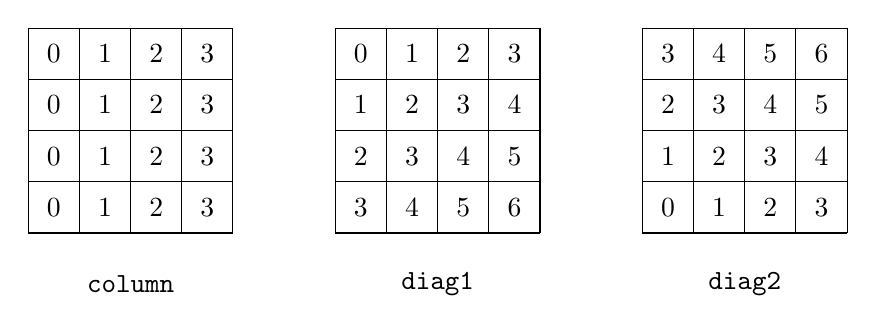
\begin{tikzpicture}[scale=.65]
  \begin{scope}
    \draw (0-6, 0) grid (4-6, 4);
    \node at (-6+0.5,3.5) {$0$};
    \node at (-6+1.5,3.5) {$1$};
    \node at (-6+2.5,3.5) {$2$};
    \node at (-6+3.5,3.5) {$3$};
    \node at (-6+0.5,2.5) {$0$};
    \node at (-6+1.5,2.5) {$1$};
    \node at (-6+2.5,2.5) {$2$};
    \node at (-6+3.5,2.5) {$3$};
    \node at (-6+0.5,1.5) {$0$};
    \node at (-6+1.5,1.5) {$1$};
    \node at (-6+2.5,1.5) {$2$};
    \node at (-6+3.5,1.5) {$3$};
    \node at (-6+0.5,0.5) {$0$};
    \node at (-6+1.5,0.5) {$1$};
    \node at (-6+2.5,0.5) {$2$};
    \node at (-6+3.5,0.5) {$3$};

    \draw (0, 0) grid (4, 4);
    \node at (0.5,3.5) {$0$};
    \node at (1.5,3.5) {$1$};
    \node at (2.5,3.5) {$2$};
    \node at (3.5,3.5) {$3$};
    \node at (0.5,2.5) {$1$};
    \node at (1.5,2.5) {$2$};
    \node at (2.5,2.5) {$3$};
    \node at (3.5,2.5) {$4$};
    \node at (0.5,1.5) {$2$};
    \node at (1.5,1.5) {$3$};
    \node at (2.5,1.5) {$4$};
    \node at (3.5,1.5) {$5$};
    \node at (0.5,0.5) {$3$};
    \node at (1.5,0.5) {$4$};
    \node at (2.5,0.5) {$5$};
    \node at (3.5,0.5) {$6$};

    \draw (6, 0) grid (10, 4);
    \node at (6.5,3.5) {$3$};
    \node at (7.5,3.5) {$4$};
    \node at (8.5,3.5) {$5$};
    \node at (9.5,3.5) {$6$};
    \node at (6.5,2.5) {$2$};
    \node at (7.5,2.5) {$3$};
    \node at (8.5,2.5) {$4$};
    \node at (9.5,2.5) {$5$};
    \node at (6.5,1.5) {$1$};
    \node at (7.5,1.5) {$2$};
    \node at (8.5,1.5) {$3$};
    \node at (9.5,1.5) {$4$};
    \node at (6.5,0.5) {$0$};
    \node at (7.5,0.5) {$1$};
    \node at (8.5,0.5) {$2$};
    \node at (9.5,0.5) {$3$};

    \node at (-4,-1) {\texttt{column}};
    \node at (2,-1) {\texttt{diag1}};
    \node at (8,-1) {\texttt{diag2}};

  \end{scope}
\end{tikzpicture}
\end{center}

$q(n)$ $n$ уәзірді $n \times n$ шахмат тақтасында
орналастыру жолдарының саны деп белгілейік.
Жоғарыдағы қайта іздеу алгоритміне сай келесі мысалды келтіре аламыз. $q(8)=92$.
% The above backtracking
% algorithm tells us that, for example, $q(8)=92$.
$n$ ұлғайған сайын ізденіс біртіндеп баяулайды,
себебі шешімдер саны  қарқынды өсіп отырады.
Мысалы, $q(16)=14772512$ мұны жоғарыда көрсетілген алгоритм көмегімен 
есептеу үшін заманауи компьютер бір минут жұмсайды
\footnote{$q(n)$-нің үлкенірек мәндерін есептеуге мүмкіндік беретін
тиімдірек алгоритм әлі табылған жоқ. Қазіргі үздік көрсеткіш -- 2016 жылы 
есептелген $q(27)=234907967154122528$ \cite{q27}.}.

\section{Ізденісті ықшамдау}

Қайта іздеу алгоритмін ізденіс дарағын
қысқарту арқылы жиі оңтайландыруға болады.
Мұндағы басты идея -- алгоритмге іздеу барысында түпкі нәтижеге қол жеткізудің мүмкін немесе мүмкін емес екендігін байқап, іздеуді одан ары жалғастыратын немесе кесіп тастай алатын ''интеллект'' қосу.
Мұндай оңтайландырудың ізденісті тиімдірек етуге
тигізетін септігі мол.

$n \times n$ тордың жоғарғы сол жақ бұрышынан
төменгі оң жақ бұрышына дейінгі жолда әр шаршыдан
бір рет қана жүріп өтетін қанша жол бар екенін іздейтін
есепті қарастырайық.
% Let us consider the problem
% of calculating the number of paths
% in an $n \times n$ grid from the upper-left corner
% to the lower-right corner such that the
% path visits each square exactly once.
Мысалы, $7 \times 7$ торда осындай 111712 жол бар.
Олардың бірі:

\begin{center}
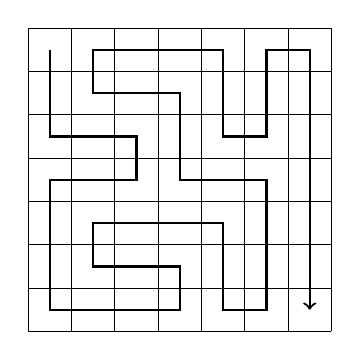
\begin{tikzpicture}[scale=.55]
  \begin{scope}
    \draw (0, 0) grid (7, 7);
    \draw[thick,->] (0.5,6.5) -- (0.5,4.5) -- (2.5,4.5) --
          (2.5,3.5) -- (0.5,3.5) -- (0.5,0.5) --
          (3.5,0.5) -- (3.5,1.5) -- (1.5,1.5) --
          (1.5,2.5) -- (4.5,2.5) -- (4.5,0.5) --
          (5.5,0.5) -- (5.5,3.5) -- (3.5,3.5) --
          (3.5,5.5) -- (1.5,5.5) -- (1.5,6.5) --
          (4.5,6.5) -- (4.5,4.5) -- (5.5,4.5) --
          (5.5,6.5) -- (6.5,6.5) -- (6.5,0.5);
  \end{scope}
\end{tikzpicture}
\end{center}

Күрделілік деңгейі біз қажет еткен деңгейге сай келгендіктен, біз $7 \times 7$ жағдайына тоқталамыз.
% We focus on the $7 \times 7$ case,
% because its level of difficulty is appropriate our needs.
Алдымен қарапайым қайта іздеу алгоритмінен бастаймыз, кейін 
ізденіс тоқтатылуы мүмкін жағдайларды байқай отырып, бірте-бірте оңтайландырамыз.
Әр оңтайландырудан кейін орындалу уақытын өлшейміз және
рекурсивті шақыруларды есептейміз. Осылайша әр оңтайландырудың
ізденіс тиімділігне тигізген септігін анық байқаймыз.

\subsubsection{Негізгі алгоритм}

Алгоритмнің алғашқы нұсқасы --  белгілі бір нәтижеге жету үшін орындалатын әрекет ету тәртібін ешқандай оңтайландырусыз сипаттайтын нұсқаулар жиынтығы.
Біз жай ғана қайта іздеу арқылы жоғарғы сол жақ бұрыштан
төменгі оң жақ бұрышқа дейінгі барлық мүмкін жолдарды құрастырып,
олардың санын есептейміз.

\begin{itemize}
\item
іске асыру уақыты: 483 секунд
\item
рекурсия шақыруларының саны: 76 миллиард
% number of recursive calls: 76 billion
\end{itemize}

\subsubsection{1-оңтайландыру}

Кез келген шешімде ең бірінші қадамды төменге, не  
оңға жасаймыз.
Бірінші жүрістен кейін әрдайым тор диагоналы бойынша
симметриялы екі жол шығады.
Мысалы, келесі жолдар симметриялы:

\begin{center}
\begin{tabular}{ccc}
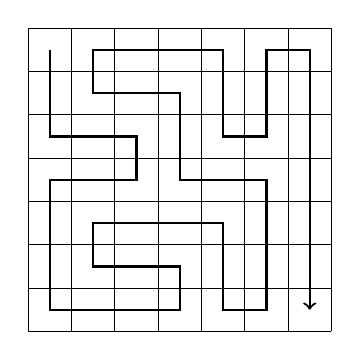
\begin{tikzpicture}[scale=.55]
  \begin{scope}
    \draw (0, 0) grid (7, 7);
    \draw[thick,->] (0.5,6.5) -- (0.5,4.5) -- (2.5,4.5) --
          (2.5,3.5) -- (0.5,3.5) -- (0.5,0.5) --
          (3.5,0.5) -- (3.5,1.5) -- (1.5,1.5) --
          (1.5,2.5) -- (4.5,2.5) -- (4.5,0.5) --
          (5.5,0.5) -- (5.5,3.5) -- (3.5,3.5) --
          (3.5,5.5) -- (1.5,5.5) -- (1.5,6.5) --
          (4.5,6.5) -- (4.5,4.5) -- (5.5,4.5) --
          (5.5,6.5) -- (6.5,6.5) -- (6.5,0.5);
  \end{scope}
\end{tikzpicture}
& \hspace{20px}
& 
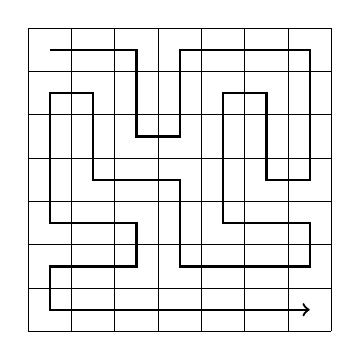
\begin{tikzpicture}[scale=.55]
  \begin{scope}[yscale=1,xscale=-1,rotate=-90]
    \draw (0, 0) grid (7, 7);
    \draw[thick,->] (0.5,6.5) -- (0.5,4.5) -- (2.5,4.5) --
          (2.5,3.5) -- (0.5,3.5) -- (0.5,0.5) --
          (3.5,0.5) -- (3.5,1.5) -- (1.5,1.5) --
          (1.5,2.5) -- (4.5,2.5) -- (4.5,0.5) --
          (5.5,0.5) -- (5.5,3.5) -- (3.5,3.5) --
          (3.5,5.5) -- (1.5,5.5) -- (1.5,6.5) --
          (4.5,6.5) -- (4.5,4.5) -- (5.5,4.5) --
          (5.5,6.5) -- (6.5,6.5) -- (6.5,0.5);
  \end{scope}
\end{tikzpicture}
\end{tabular}
\end{center}

Осылайша әрдайым алдымен төмен (не оңға) бір қадам қозғалып,
шешімдер санын екіге көбейтеміз.

\begin{itemize}
\item
іске асыру уақыты: 244 секунд
\item
рекурсия шақыруларының саны: 38 миллиард
\end{itemize}

\subsubsection{2-оңтайландыру}

Егер тордағы барлық шаршыларды өтпестен
оң жақ төменгі бұрышқа жетсек, бұл шешімнің
толық болмайтындығы анық.
Мұндай жол үлгісі төмендегідей болады:

\begin{center}
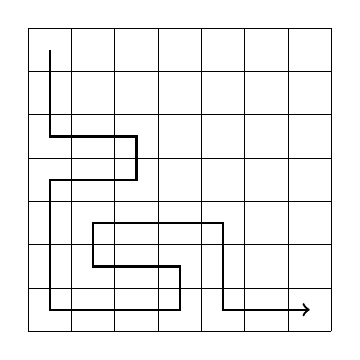
\begin{tikzpicture}[scale=.55]
  \begin{scope}
    \draw (0, 0) grid (7, 7);
    \draw[thick,->] (0.5,6.5) -- (0.5,4.5) -- (2.5,4.5) --
          (2.5,3.5) -- (0.5,3.5) -- (0.5,0.5) --
          (3.5,0.5) -- (3.5,1.5) -- (1.5,1.5) --
          (1.5,2.5) -- (4.5,2.5) -- (4.5,0.5) --
          (6.5,0.5);
  \end{scope}
\end{tikzpicture}
\end{center}
Осындай бақылауларды қолдана отырып, оң жақ төменгі бұрышқа
тым ерте жеткен жағдайда ізденісті бірден тоқтатамыз.
\begin{itemize}
\item
іске асыру уақыты: 119 секунд
\item
рекурсия шақыруларының саны: 20 миллиард
\end{itemize}

\subsubsection{3-оңтайландыру}
    
Жол шекараға жетіп, не солға, не оңға 
бағыт ала алса, тор әлі болмаған шаршыларды қамтитын
екі бөлікке бөлінеді.
Мысалы, келесі жағдайда жол оңға, не солға бағыт ала алады:

\begin{center}
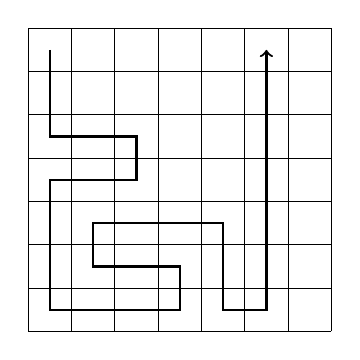
\begin{tikzpicture}[scale=.55]
  \begin{scope}
    \draw (0, 0) grid (7, 7);
    \draw[thick,->] (0.5,6.5) -- (0.5,4.5) -- (2.5,4.5) --
          (2.5,3.5) -- (0.5,3.5) -- (0.5,0.5) --
          (3.5,0.5) -- (3.5,1.5) -- (1.5,1.5) --
          (1.5,2.5) -- (4.5,2.5) -- (4.5,0.5) --
          (5.5,0.5) -- (5.5,6.5);
  \end{scope}
\end{tikzpicture}
\end{center}
Бұл жағдайда біз барлық шаршыларға бара алмаймыз,
сол себепті ізденісті ықшамдап аламыз.
Бұл оңтайландыру аса пайдалы:

\begin{itemize}
\item
іске асыру уақыты: 1.8 секунд
\item
рекурсия шақыруларының саны: 221 миллион
\end{itemize} 

\subsubsection{4-оңтайландыру}

3-оңтайландырудың идеясын былайша жалпылай аламыз:
егер жол жалғаса алмаса, бірақ сол не оңға
бағыт ала алса, тор әлі болмаған шаршыларды
қамтитын екі бөлікке бөлінеді. Мысалы, төмендегідей жол:

\begin{center}
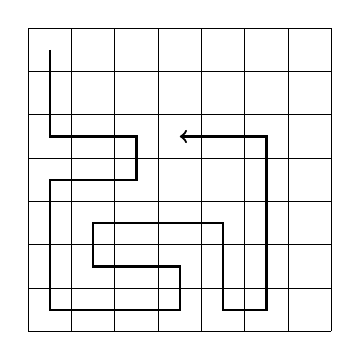
\begin{tikzpicture}[scale=.55]
  \begin{scope}
    \draw (0, 0) grid (7, 7);
    \draw[thick,->] (0.5,6.5) -- (0.5,4.5) -- (2.5,4.5) --
          (2.5,3.5) -- (0.5,3.5) -- (0.5,0.5) --
          (3.5,0.5) -- (3.5,1.5) -- (1.5,1.5) --
          (1.5,2.5) -- (4.5,2.5) -- (4.5,0.5) --
          (5.5,0.5) -- (5.5,4.5) -- (3.5,4.5);
  \end{scope}
\end{tikzpicture}
\end{center}
Енді барлық шаршыларға бара алмайтынымыз анық, сондықтан ізденісті тоқтатамыз.
Мұндай оңтайландырудан кейін ізденіс өте тиімді болмақ:

\begin{itemize}
\item
іске асыру уақыты: 0.6 секунд
\item
рекурсия шақыруларының саны: 69 миллион
\end{itemize}

~\\
Осы жерден алгоритмді оңтайландыруды тоқтатып,
қандай нәтижеге қол жеткізгенімізді көрейік.
Бастапқы алгоритмнің іске асыру уақыты 483 секунд болса,
оңтайландырулардан кейінгі іске асыру уақыты -- небәрі 0.6 секунд.
Осылайша оңтайландырудың әсерінен алгоритмнің жылдамдығы шамамен 1000 есеге артады.

Бұл қайта іздеудегі әдепкі құбылыс,
себебі ізденіс дарағы әдетте үлкен болып келеді және кішкене
бақылаулардың өзі ізденісті тиімді ықшамдайды.
Әсіресе алгоритмнің алғашқы қадамдарында, яки 
ізденіс дарағының басында орын 
алатын оңтайландырулар өте пайдалы болмақ.

\section{Ортада кездесу}

\index{ортада кездесу}

\key{Ортада кездесу} (meet in the middle) --
ізденіс аясын екі тең бөлікке бөлу тәсілі.
Мұнда екі бөлікке де дербес ізденіс жүргізіліп,
соңында ізденіс нәтижелері қосылады.

Бұл тәсілді ізденіс нәтижелерін тиімді қосу мүмкіндігі
болған жағдайда қолдана аламыз.
Демек екі ізденіс бір үлкен ізденіске қарағанда аз уақытты талап етуі мүмкін.
Әдетте ортада кездесу тәсілін қолдана отырып, $2^n$ факторын $2^{n/2}$ факторына айналдыра аламыз.

Үлгі ретінде $n$ саннан тұратын тізім мен $x$ саны берілген есепті қарастырайық.
Тапсырма бойынша тізімдегі қандай да бір сандар қосындысынан $x$ санын алуға болатынын анықтау керек.
Мысалы, $[2,4,5,9]$ тізбегі мен $x=15$ саны берілген,
$[2,4,9]$ сандарын таңдау арқылы $2+4+9=15$ ала аламыз.
Бірақ $x=10$ болған жағдайда дәл осы тізіммен қосындыға қол жеткізу мүмкін болмас еді.

Қарапайым алгоритм -- барлық ішжиындармен өтіп шығып, 
қосындысы $x$ болатынын тексеру.
Мұндай алгоритмнің уақытша күрделілігі -- $O(2^n)$,
себебі $O(2^n)$ ішжиыны бар. Дегенмен ортада кездесу тәсілін қолдана отырып,
тиімдірек $O(2^{n/2})$ уақытына\footnote{Бұл идеяны 1974 жылы Э.Горовиц пен С.Сахни  
таныстырған болатын\cite{hor74}.} қол жеткізе аламыз.
$O(2^n)$ мен $O(2^{n/2})$ әртүрлі уақытша күрделіліктері екендігін ескерген жөн,
себебі $2^{n/2}$ $\sqrt{2^n}$ тең.

Мұндағы идея -- тізімді $A$ және $B$ тізімдеріне 
тең элемент санын қамтитындай етіп бөлу.
Бірірнші ізденіс $A$-ның барлық ішжиындарын
құрайды және олардың қосындыларын $S_A$ тізімінде сақтайды.
Екінші ізденіс сәйкесінше $S_B$ тізімін $B$-дан құрайды. 
Бұдан кейін $S_A$-дан бір элемент, $S_B$-дан бір элемент қана алу арқылы 
$x$ санын құрау мүмкіндігін тексеру жеткілікті.
Бұл бастапқы тізімдегі сандардан $x$ қосындысын құрауға болатын жағдайда ғана  мүмкін болмақ.

Мысалы, тізім -- $[2,4,5,9]$, ал $x=15$.
Алдымен екі тізімге бөліп аламыз: $A=[2,4]$ және $B=[5,9]$.
Кейін $S_A=[0,2,4,6]$ мен $S_B=[0,5,9,14]$ тізімдерін құрамыз.
Бұл жағдайда $x=15$-ті құрау мүмкін, себебі $S_A$ $6$ қосындысын қамтиды,
ал $S_B$ $9$ мәнін қамтиды, сонда $6+9=15$ болады.
Бұл $[2,4,9]$ шешіміне сәйкес келеді.

Біз алгоритмді уақытша күрделілігі $O(2^{n/2})$ болатындай
жүзеге асыра аламыз.
Біріншіден \emph{сұрыпталған} $S_A$ және $S_B$ тізімдерін құраймыз,
ол $O(2^{n/2})$ уақытында бірігу тәсілін қолдану арқылы жүзеге асырылады.
Бұдан кейін тізімдер сұрыпталғандықтан $S_A$ мен $S_B$ тізмдерінен 
$x$ қосындысын құрауға болатындығын $O(2^{n/2})$ уақытында тексере аламыз.